\chapter{Nasazení}

K testování a provozu webové aplikace jsem získál virtualizovaný server, ke~kterému přistupuji pomocí SSH
\footnote{Program, který komunikuje zabezpečeným komunikačním protokolem. Používá TCP/IP.}.

\subsection*{Virtuální privátní server}

Jde o server běžící na virtualizovaném hardwaru a~často se označuje zkratkou VPS.
Bývá poskytován hostingovými společnostmi, které svůj fyzický stroj nabízejí více klientům najednou.
Každému zákazníkovi vymezí prostor s~vlastní instancí operačního systému, jednotlivými hostingovými službami
a~vlastní konfigurací. Nevýhodu je sdílení fyzických prostředků, poněvadž při~nedostatečném nastavení
může docházet k~ovlivňování cizích VPS. Výhodou je naopak levnější pořízení ve~srovnání celého fyzického serveru.

\section{Softwarové požadavky}

Aplikace běží na VPS s OS Ubuntu~\cite{ubuntu} verze 15.10. Na veřejné adrese virtualního serveru
je dostupná RESTová webová služba Catcher, s níž může zvnějšku komunikovat libovolná aplikace,
která disponuje HTTP protokolem a dostupností běžného portu 80. Jako prostředník mezi klientskou aplikací
a~uWSGI~2.0.12~\cite{python_uwsgi}, jehož úkolem je udržovat Catchera, zde běží webový server Nginx 1.9.3.
Data se ukládají na databázový server MySQL verze 5.6.28.

Pro běh aplikace byly stáhnuty všechny potřebné balíčky včetně pipu~\cite{python_pip},
jenž slouží pro správu nesystémových knihoven v Pythonu. Detailní seznam všech zásvislostí obsahuje soubor
\texttt{README.md}, uložený v rodičovském adresáři projektu. Lepší správu souborů na serveru mi pak zajistil program Midnight Commander~\cite{mc}.

\begin{figure}[ht!]
\centering
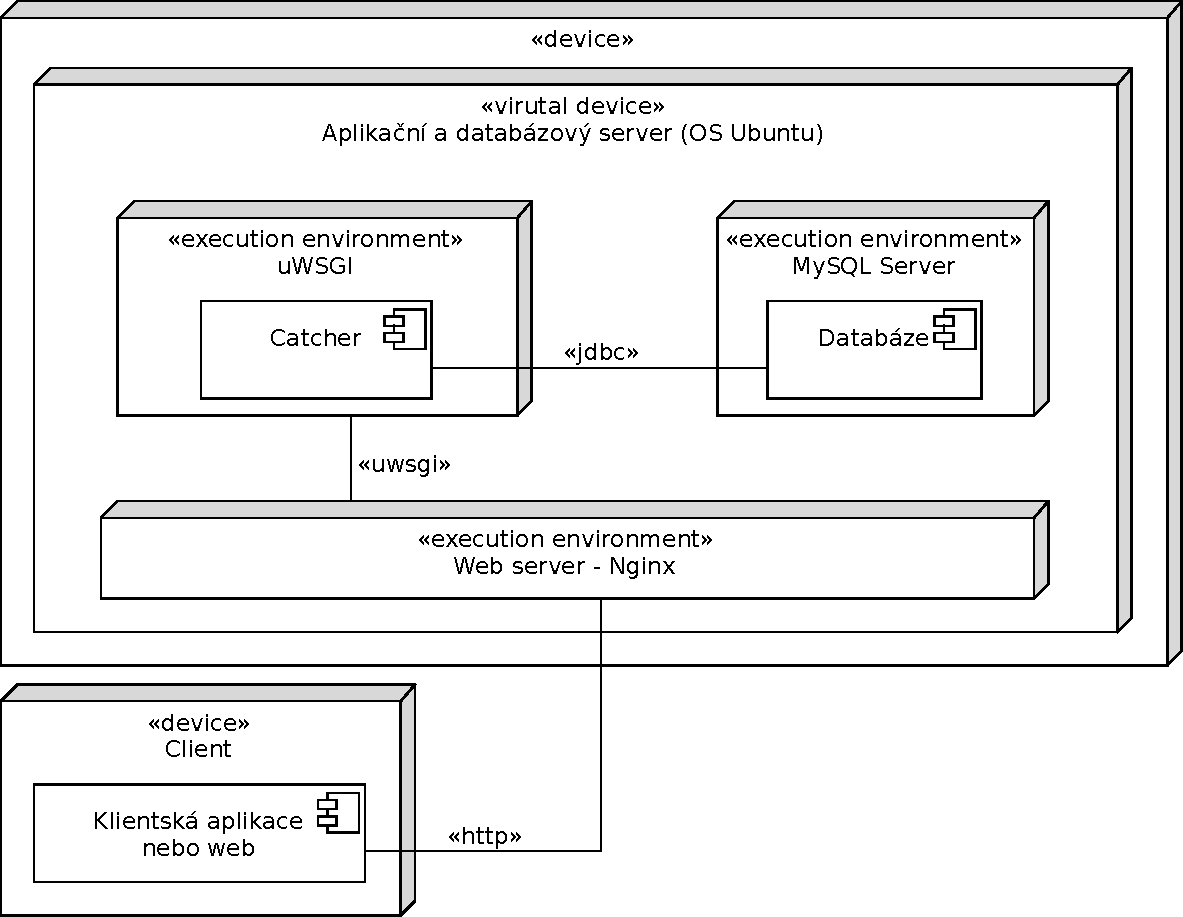
\includegraphics[width=130mm]{./images/diagram-nasazeni.pdf}
\caption{Diagram nasazení\label{overflow}}
\end{figure}

\section{uWSGI}

Aby bylo lépe pochopitelné zapojení uWSGI do celého procesu nasazení, popíšeme si jej trochu detailněji.

Projekt uWSGI je malý program, který se stará o management procesu aplikace.
Funguje jako prostředník mezi webovým serverem a aplikací,
se kterými komunikuje vlastním uwsgi protokolem, respektive standartním WSGI.
Detail komunikace je vidět na obrázku~\ref{fig:uwsgi}.

\begin{figure}[ht!]
\centering

\includegraphics[width=135mm]{./images/uwsgi.pdf}
\caption{Komunikace mezi webovým serverem a aplikací v Pythonu; zdroj:~autor na základě~\cite{uwsgi}\label{overflow}}
\label{fig:uwsgi}
\end{figure}

\subsection*{uWSGI úloha}

Spuštění webové aplikace provadím následujícím příkazem. Proces poslouchá na~portu 8080 a~po~celou dobu běží na~pozadí.

\begingroup
\fontsize{9.5pt}{11pt}\selectfont
\begin{verbatim}
$ uwsgi --socket localhost:8080 --wsgi-file ./restapi.py --callable api &
\end{verbatim}
\endgroup

\section{Konfigurace}

\subsection*{Konfigurační soubor}

Protože všechny moje zdrojové kódy byly zveřejněny v repozitáři na GitHubu, nebylo by správné, aby obsahovaly jakákoliv hesla.
Pro tyto potřeby byl vytvořen konfigurační soubor, který mám zazálohovaný na vlastním cloudovém uložišti
a~pomocí programu wget~\cite{wget} si jej stahuju do~projektu vždy, když je změněn.
Tento konfigurační soubor obsahuje hesla k~produkční a~testovací databázi
nebo k~emailovému účtu, který používám pro~obnovu hesla uživatelů.

\subsection*{Databáze}

Pro přístup do databáze bylo potřeba vytvořit uživatele s právem zapisovat, číst a mazat.
Tento účet se nadále autentizuje heslem, které je uložené v konfiguračním souboru.
Příkazy pro vytvoření uživatele v SQL jsou následující:

\begingroup
\fontsize{9.5pt}{11pt}\selectfont
\begin{verbatim}
CREATE USER 'catcher-server'@'localhost' IDENTIFIED BY 'tajne_heslo';
GRANT SELECT, INSERT, UPDATE, DELETE
    ON catcher. * TO 'catcher-server'@'localhost';
\end{verbatim}
\endgroup

\subsection*{Nginx}

Protože disponuji pouze jednou veřejnou adresou na VPS, bylo potřeba webový server nakonfigurovat tak,
aby dokázal obsluhovat požadavky webové aplikace i požadavky
na zobrazení dokumentace. Konfigurace na serveru byla následující:

\begingroup
\fontsize{9.5pt}{11pt}\selectfont
\begin{verbatim}
upstream catcher_uwsgi {
    # adresa a port, na které přeposílám požadavky pro Catchera
    server localhost:8080;
}

server {
    # číslo portu na ipv4
    listen       80;
    # číslo portu na ipv6
    listen       [::]:80;
    # jméno serveru
    server_name  catcher.zlutazimnice.cz *.catcher.zlutazimnice.cz;
    charset      utf-8;
    index        index.html;
    
    # maximální velikost uploadu
    client_max_body_size 75M;

    # dokumentace na catcher.zlutazimnice.cz
    location / {
        # adresář s obsahem webu
        root   /var/www/catcher;
    }

    # webová aplikace na catcher.zlutazimnice.cz/api
    location /api {
        include     uwsgi_params;
        # upstream pro spojení s uwsgi
        uwsgi_pass  catcher_uwsgi;
    }
}
\end{verbatim}
\endgroup

Pro vývoj na svém počítači jsem použil trochu odlišnou konfiguraci, protože
jsem nemusel na jedné adrese provozovat dokumentaci i aplikaci.
V prvních fázích vývoje jsem dokonce ani Nginx používat nemusel, protože uWSGI umožňuje simulovat
chování webového serveru.
Pro produkční nasazení ale~není tento postup doporučen.

\section{Údržba}

Standartem pro větší aplikace by měl být monitorovací systém,
který sleduje zátěž jednotlivých komponent (webová aplikace, databáze, webový server atd.)
a~v~případě výpadku informuje administrátora SMS zprávou nebo emailem.
Pro potřeby Catchera jsem však využil daleko jednodušího řešení -- webové aplikace Uptime Robot~\cite{uptime_robot},
která v pravidelných intervalech \uv{oťukává} mnou definovavné adresy a~ověřuje jejich dostupnost.
Pro použití v~omezené míře je zdarma a~v~sitauci, kdy je Catcher nedostupný, mě informuje emailem.


%by mělo stačit \uv{oťukávání} z testovacíh

%~\cite{uptime_robot}


%Pro potřeby Catchera by mělo stačit \uv{oťukávání} z testovacíh

%Až bude Catcher nasazen do ostrého provozu, pro jeho potřeby by měl stačit Cron\footnote{Jde o softwarového démona, který slouží
%k~automatickému spouštění periodicky se opakujících příkazů a procesů.},
%který by v~pravidelných intervalech \uv{oťukával} aplikaci a~stanovil, zda korektně běží.

Dále je nutné pro případ výpadku pravidelně zálohovat databázi. Místo manuálního zálohování programem
\texttt{mysqldump}~\cite{mysqldump}, lze použít Cron\footnote{Jde o softwarového démona, který slouží
k~automatickému spouštění periodicky se opakujících příkazů a procesů.}, který by pravidelně tento program spouštěl. 
V~případě výpadku by tak stačilo aplikaci opravit a~nahrát poslední zálohu.
Catcher aktuálně disponuje pouze manuálním zálohováním databáze.



% TODO: IDEA: Pouzit nasledujici:

%\section{Co by šlo udělat lépe}
%Během vývoje jsem se setkal se zajímavými nástroji, na které v tomto projektu nezbyla kapacita. Jejih použití by přineslo několik zlepšení, proto jsem se rozhodl je zde uvést:
%list:
%Virtualenv, Codevoc, Travis CI
%IDEA: Lze se zminit o testovani a prubezne integraci. Napriklad napsat, ze mame zajem v budoucnu pouzivat Codevoc (mozna spis testovani) nebo Travis CI.